\documentclass[1p]{elsarticle_modified}
%\bibliographystyle{elsarticle-num}

%\usepackage[colorlinks]{hyperref}
%\usepackage{abbrmath_seonhwa} %\Abb, \Ascr, \Acal ,\Abf, \Afrak
\usepackage{amsfonts}
\usepackage{amssymb}
\usepackage{amsmath}
\usepackage{amsthm}
\usepackage{scalefnt}
\usepackage{amsbsy}
\usepackage{kotex}
\usepackage{caption}
\usepackage{subfig}
\usepackage{color}
\usepackage{graphicx}
\usepackage{xcolor} %% white, black, red, green, blue, cyan, magenta, yellow
\usepackage{float}
\usepackage{setspace}
\usepackage{hyperref}

\usepackage{tikz}
\usetikzlibrary{arrows}

\usepackage{multirow}
\usepackage{array} % fixed length table
\usepackage{hhline}

%%%%%%%%%%%%%%%%%%%%%
\makeatletter
\renewcommand*\env@matrix[1][\arraystretch]{%
	\edef\arraystretch{#1}%
	\hskip -\arraycolsep
	\let\@ifnextchar\new@ifnextchar
	\array{*\c@MaxMatrixCols c}}
\makeatother %https://tex.stackexchange.com/questions/14071/how-can-i-increase-the-line-spacing-in-a-matrix
%%%%%%%%%%%%%%%

\usepackage[normalem]{ulem}

\newcommand{\msout}[1]{\ifmmode\text{\sout{\ensuremath{#1}}}\else\sout{#1}\fi}
%SOURCE: \msout is \stkout macro in https://tex.stackexchange.com/questions/20609/strikeout-in-math-mode

\newcommand{\cancel}[1]{
	\ifmmode
	{\color{red}\msout{#1}}
	\else
	{\color{red}\sout{#1}}
	\fi
}

\newcommand{\add}[1]{
	{\color{blue}\uwave{#1}}
}

\newcommand{\replace}[2]{
	\ifmmode
	{\color{red}\msout{#1}}{\color{blue}\uwave{#2}}
	\else
	{\color{red}\sout{#1}}{\color{blue}\uwave{#2}}
	\fi
}

\newcommand{\Sol}{\mathcal{S}} %segment
\newcommand{\D}{D} %diagram
\newcommand{\A}{\mathcal{A}} %arc


%%%%%%%%%%%%%%%%%%%%%%%%%%%%%5 test

\def\sl{\operatorname{\textup{SL}}(2,\Cbb)}
\def\psl{\operatorname{\textup{PSL}}(2,\Cbb)}
\def\quan{\mkern 1mu \triangleright \mkern 1mu}

\theoremstyle{definition}
\newtheorem{thm}{Theorem}[section]
\newtheorem{prop}[thm]{Proposition}
\newtheorem{lem}[thm]{Lemma}
\newtheorem{ques}[thm]{Question}
\newtheorem{cor}[thm]{Corollary}
\newtheorem{defn}[thm]{Definition}
\newtheorem{exam}[thm]{Example}
\newtheorem{rmk}[thm]{Remark}
\newtheorem{alg}[thm]{Algorithm}

\newcommand{\I}{\sqrt{-1}}
\begin{document}

%\begin{frontmatter}
%
%\title{Boundary parabolic representations of knots up to 8 crossings}
%
%%% Group authors per affiliation:
%\author{Yunhi Cho} 
%\address{Department of Mathematics, University of Seoul, Seoul, Korea}
%\ead{yhcho@uos.ac.kr}
%
%
%\author{Seonhwa Kim} %\fnref{s_kim}}
%\address{Center for Geometry and Physics, Institute for Basic Science, Pohang, 37673, Korea}
%\ead{ryeona17@ibs.re.kr}
%
%\author{Hyuk Kim}
%\address{Department of Mathematical Sciences, Seoul National University, Seoul 08826, Korea}
%\ead{hyukkim@snu.ac.kr}
%
%\author{Seokbeom Yoon}
%\address{Department of Mathematical Sciences, Seoul National University, Seoul, 08826,  Korea}
%\ead{sbyoon15@snu.ac.kr}
%
%\begin{abstract}
%We find all boundary parabolic representation of knots up to 8 crossings.
%
%\end{abstract}
%\begin{keyword}
%    \MSC[2010] 57M25 
%\end{keyword}
%
%\end{frontmatter}

%\linenumbers
%\tableofcontents
%
\newcommand\colored[1]{\textcolor{white}{\rule[-0.35ex]{0.8em}{1.4ex}}\kern-0.8em\color{red} #1}%
%\newcommand\colored[1]{\textcolor{white}{ #1}\kern-2.17ex	\textcolor{white}{ #1}\kern-1.81ex	\textcolor{white}{ #1}\kern-2.15ex\color{red}#1	}

{\Large $\underline{12n_{0873}~(K12n_{0873})}$}

\setlength{\tabcolsep}{10pt}
\renewcommand{\arraystretch}{1.6}
\vspace{1cm}\begin{tabular}{m{100pt}>{\centering\arraybackslash}m{274pt}}
\multirow{5}{120pt}{
	\centering
	\includegraphics[width=112pt]{../../../GIT/diagram.site/Diagrams/png/2962_12n_0873.png}\\
\ \ \ A knot diagram\footnotemark}&
\allowdisplaybreaks
\textbf{Linearized knot diagam} \\
\cline{2-2}
 &
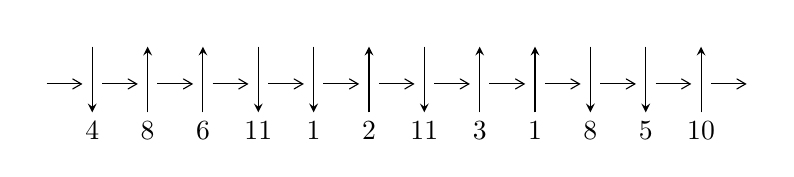
\begin{tikzpicture}[x=20pt, y=17pt]
	% nodes
	\node (C0) at (0, 0) {};
	\node (C1) at (1, 0) {};
	\node (C1U) at (1, +1) {};
	\node (C1D) at (1, -1) {4};

	\node (C2) at (2, 0) {};
	\node (C2U) at (2, +1) {};
	\node (C2D) at (2, -1) {8};

	\node (C3) at (3, 0) {};
	\node (C3U) at (3, +1) {};
	\node (C3D) at (3, -1) {6};

	\node (C4) at (4, 0) {};
	\node (C4U) at (4, +1) {};
	\node (C4D) at (4, -1) {11};

	\node (C5) at (5, 0) {};
	\node (C5U) at (5, +1) {};
	\node (C5D) at (5, -1) {1};

	\node (C6) at (6, 0) {};
	\node (C6U) at (6, +1) {};
	\node (C6D) at (6, -1) {2};

	\node (C7) at (7, 0) {};
	\node (C7U) at (7, +1) {};
	\node (C7D) at (7, -1) {11};

	\node (C8) at (8, 0) {};
	\node (C8U) at (8, +1) {};
	\node (C8D) at (8, -1) {3};

	\node (C9) at (9, 0) {};
	\node (C9U) at (9, +1) {};
	\node (C9D) at (9, -1) {1};

	\node (C10) at (10, 0) {};
	\node (C10U) at (10, +1) {};
	\node (C10D) at (10, -1) {8};

	\node (C11) at (11, 0) {};
	\node (C11U) at (11, +1) {};
	\node (C11D) at (11, -1) {5};

	\node (C12) at (12, 0) {};
	\node (C12U) at (12, +1) {};
	\node (C12D) at (12, -1) {10};
	\node (C13) at (13, 0) {};

	% arrows
	\draw[->,>={angle 60}]
	(C0) edge (C1) (C1) edge (C2) (C2) edge (C3) (C3) edge (C4) (C4) edge (C5) (C5) edge (C6) (C6) edge (C7) (C7) edge (C8) (C8) edge (C9) (C9) edge (C10) (C10) edge (C11) (C11) edge (C12) (C12) edge (C13) ;	\draw[->,>=stealth]
	(C1U) edge (C1D) (C2D) edge (C2U) (C3D) edge (C3U) (C4U) edge (C4D) (C5U) edge (C5D) (C6D) edge (C6U) (C7U) edge (C7D) (C8D) edge (C8U) (C9D) edge (C9U) (C10U) edge (C10D) (C11U) edge (C11D) (C12D) edge (C12U) ;
	\end{tikzpicture} \\
\hhline{~~} \\& 
\textbf{Solving Sequence} \\ \cline{2-2} 
 &
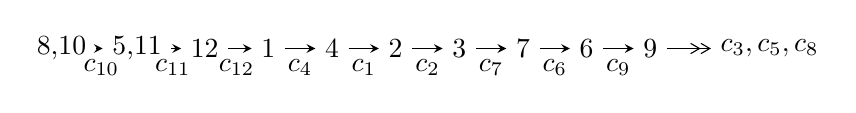
\begin{tikzpicture}[x=23pt, y=7pt]
	% node
	\node (A0) at (-1/8, 0) {8,10};
	\node (A1) at (17/16, 0) {5,11};
	\node (A2) at (17/8, 0) {12};
	\node (A3) at (25/8, 0) {1};
	\node (A4) at (33/8, 0) {4};
	\node (A5) at (41/8, 0) {2};
	\node (A6) at (49/8, 0) {3};
	\node (A7) at (57/8, 0) {7};
	\node (A8) at (65/8, 0) {6};
	\node (A9) at (73/8, 0) {9};
	\node (C1) at (1/2, -1) {$c_{10}$};
	\node (C2) at (13/8, -1) {$c_{11}$};
	\node (C3) at (21/8, -1) {$c_{12}$};
	\node (C4) at (29/8, -1) {$c_{4}$};
	\node (C5) at (37/8, -1) {$c_{1}$};
	\node (C6) at (45/8, -1) {$c_{2}$};
	\node (C7) at (53/8, -1) {$c_{7}$};
	\node (C8) at (61/8, -1) {$c_{6}$};
	\node (C9) at (69/8, -1) {$c_{9}$};
	\node (A10) at (11, 0) {$c_{3},c_{5},c_{8}$};

	% edge
	\draw[->,>=stealth]	
	(A0) edge (A1) (A1) edge (A2) (A2) edge (A3) (A3) edge (A4) (A4) edge (A5) (A5) edge (A6) (A6) edge (A7) (A7) edge (A8) (A8) edge (A9) ;
	\draw[->>,>={angle 60}]	
	(A9) edge (A10);
\end{tikzpicture} \\ 

\end{tabular} \\

\footnotetext{
The image of knot diagram is generated by the software ``\textbf{Draw programme}" developed by Andrew Bartholomew(\url{http://www.layer8.co.uk/maths/draw/index.htm\#Running-draw}), where we modified some parts for our purpose(\url{https://github.com/CATsTAILs/LinksPainter}).
}\phantom \\ \newline 
\centering \textbf{Ideals for irreducible components\footnotemark of $X_{\text{par}}$} 
 
\begin{align*}
I^u_{1}&=\langle 
-14522454433989 u^{21}-25681776487073 u^{20}+\cdots+3586941656707 b-31211211235135,\\
\phantom{I^u_{1}}&\phantom{= \langle  }-36929494073687 u^{21}-51455949517906 u^{20}+\cdots+7173883313414 a-58527943826811,\\
\phantom{I^u_{1}}&\phantom{= \langle  }u^{22}+u^{21}+\cdots+11 u^2-1\rangle \\
I^u_{2}&=\langle 
4.95406\times10^{129} u^{47}-1.26151\times10^{130} u^{46}+\cdots+1.96857\times10^{131} b-1.02263\times10^{133},\\
\phantom{I^u_{2}}&\phantom{= \langle  }4.32742\times10^{130} u^{47}-2.32616\times10^{130} u^{46}+\cdots+1.83077\times10^{133} a+1.08093\times10^{134},\\
\phantom{I^u_{2}}&\phantom{= \langle  }u^{48}-3 u^{47}+\cdots-5967 u+837\rangle \\
I^u_{3}&=\langle 
4.59095\times10^{33} u^{27}+3.06795\times10^{34} u^{26}+\cdots+1.27873\times10^{34} b-2.02070\times10^{34},\\
\phantom{I^u_{3}}&\phantom{= \langle  }5.39233\times10^{33} u^{27}+3.74664\times10^{34} u^{26}+\cdots+1.27873\times10^{34} a+1.86540\times10^{33},\;u^{28}+6 u^{27}+\cdots-3 u+1\rangle \\
I^u_{4}&=\langle 
b- u-1,\;a+1,\;u^2+u+1\rangle \\
I^u_{5}&=\langle 
b,\;a^2- a-1,\;u-1\rangle \\
\\
\end{align*}
\raggedright * 5 irreducible components of $\dim_{\mathbb{C}}=0$, with total 102 representations.\\
\footnotetext{All coefficients of polynomials are rational numbers. But the coefficients are sometimes approximated in decimal forms when there is not enough margin.}
\newpage
\renewcommand{\arraystretch}{1}
\centering \section*{I. $I^u_{1}= \langle -1.45\times10^{13} u^{21}-2.57\times10^{13} u^{20}+\cdots+3.59\times10^{12} b-3.12\times10^{13},\;-3.69\times10^{13} u^{21}-5.15\times10^{13} u^{20}+\cdots+7.17\times10^{12} a-5.85\times10^{13},\;u^{22}+u^{21}+\cdots+11 u^2-1 \rangle$}
\flushleft \textbf{(i) Arc colorings}\\
\begin{tabular}{m{7pt} m{180pt} m{7pt} m{180pt} }
\flushright $a_{8}=$&$\begin{pmatrix}0\\u\end{pmatrix}$ \\
\flushright $a_{10}=$&$\begin{pmatrix}1\\0\end{pmatrix}$ \\
\flushright $a_{5}=$&$\begin{pmatrix}5.14777 u^{21}+7.17268 u^{20}+\cdots+31.1983 u+8.15847\\4.04870 u^{21}+7.15980 u^{20}+\cdots+19.2083 u+8.70134\end{pmatrix}$ \\
\flushright $a_{11}=$&$\begin{pmatrix}1\\u^2\end{pmatrix}$ \\
\flushright $a_{12}=$&$\begin{pmatrix}-1.60242 u^{21}-2.95306 u^{20}+\cdots-16.8212 u-10.3165\\-1.34149 u^{21}-3.53682 u^{20}+\cdots+5.21457 u+1.60180\end{pmatrix}$ \\
\flushright $a_{1}=$&$\begin{pmatrix}-2.94390 u^{21}-6.48988 u^{20}+\cdots-11.6066 u-8.71475\\-1.34149 u^{21}-3.53682 u^{20}+\cdots+5.21457 u+1.60180\end{pmatrix}$ \\
\flushright $a_{4}=$&$\begin{pmatrix}7.46458 u^{21}+11.2167 u^{20}+\cdots+45.2589 u+14.8349\\5.25346 u^{21}+9.78267 u^{20}+\cdots+21.5251 u+10.4285\end{pmatrix}$ \\
\flushright $a_{2}=$&$\begin{pmatrix}0.808188 u^{21}+0.198874 u^{20}+\cdots+3.22832 u-1.25017\\3.18771 u^{21}+5.17826 u^{20}+\cdots+15.6431 u+6.85526\end{pmatrix}$ \\
\flushright $a_{3}=$&$\begin{pmatrix}0.808188 u^{21}+0.198874 u^{20}+\cdots+3.22832 u-1.25017\\3.75209 u^{21}+6.68875 u^{20}+\cdots+14.8349 u+7.46458\end{pmatrix}$ \\
\flushright $a_{7}=$&$\begin{pmatrix}u\\u^3+u\end{pmatrix}$ \\
\flushright $a_{6}=$&$\begin{pmatrix}-5.04727 u^{21}-8.95412 u^{20}+\cdots-17.3452 u-2.58840\\0.141857 u^{21}-1.92509 u^{20}+\cdots+17.6199 u+3.65407\end{pmatrix}$ \\
\flushright $a_{9}=$&$\begin{pmatrix}-0.597562 u^{21}-0.425433 u^{20}+\cdots-9.43715 u-7.53117\\-5.64484 u^{21}-9.37955 u^{20}+\cdots-26.7823 u-10.1196\end{pmatrix}$\\&\end{tabular}
\flushleft \textbf{(ii) Obstruction class $= -1$}\\~\\
\flushleft \textbf{(iii) Cusp Shapes $= -\frac{10307681188458}{3586941656707} u^{21}-\frac{33226595290622}{3586941656707} u^{20}+\cdots+\frac{96107874232352}{3586941656707} u+\frac{30375267725218}{3586941656707}$}\\~\\
\newpage\renewcommand{\arraystretch}{1}
\flushleft \textbf{(iv) u-Polynomials at the component}\newline \\
\begin{tabular}{m{50pt}|m{274pt}}
Crossings & \hspace{64pt}u-Polynomials at each crossing \\
\hline $$\begin{aligned}c_{1},c_{7},c_{10}\end{aligned}$$&$\begin{aligned}
&u^{22}+u^{21}+\cdots+11 u^2-1
\end{aligned}$\\
\hline $$\begin{aligned}c_{2},c_{8}\end{aligned}$$&$\begin{aligned}
&u^{22}+6 u^{21}+\cdots+228 u+52
\end{aligned}$\\
\hline $$\begin{aligned}c_{3},c_{9},c_{12}\end{aligned}$$&$\begin{aligned}
&u^{22}- u^{21}+\cdots+11 u^2-1
\end{aligned}$\\
\hline $$\begin{aligned}c_{4},c_{11}\end{aligned}$$&$\begin{aligned}
&u^{22}-6 u^{21}+\cdots-228 u+52
\end{aligned}$\\
\hline $$\begin{aligned}c_{5}\end{aligned}$$&$\begin{aligned}
&u^{22}-8 u^{20}+\cdots-7 u+1
\end{aligned}$\\
\hline $$\begin{aligned}c_{6}\end{aligned}$$&$\begin{aligned}
&u^{22}-8 u^{20}+\cdots+7 u+1
\end{aligned}$\\
\hline
\end{tabular}\\~\\
\newpage\renewcommand{\arraystretch}{1}
\flushleft \textbf{(v) Riley Polynomials at the component}\newline \\
\begin{tabular}{m{50pt}|m{274pt}}
Crossings & \hspace{64pt}Riley Polynomials at each crossing \\
\hline $$\begin{aligned}c_{1},c_{3},c_{7}\\c_{9},c_{10},c_{12}\end{aligned}$$&$\begin{aligned}
&y^{22}-17 y^{21}+\cdots-22 y+1
\end{aligned}$\\
\hline $$\begin{aligned}c_{2},c_{4},c_{8}\\c_{11}\end{aligned}$$&$\begin{aligned}
&y^{22}-10 y^{21}+\cdots-5184 y+2704
\end{aligned}$\\
\hline $$\begin{aligned}c_{5},c_{6}\end{aligned}$$&$\begin{aligned}
&y^{22}-16 y^{21}+\cdots-23 y+1
\end{aligned}$\\
\hline
\end{tabular}\\~\\
\newpage\flushleft \textbf{(vi) Complex Volumes and Cusp Shapes}
$$\begin{array}{c|c|c}  
\text{Solutions to }I^u_{1}& \I (\text{vol} + \sqrt{-1}CS) & \text{Cusp shape}\\
 \hline 
\begin{aligned}
u &= \phantom{-}0.273252 + 1.034170 I \\
a &= -0.328090 + 1.002630 I \\
b &= \phantom{-}0.35769 - 1.45925 I\end{aligned}
 & \phantom{-}5.13893 + 2.17267 I & \phantom{-}4.11172 - 1.64759 I \\ \hline\begin{aligned}
u &= \phantom{-}0.273252 - 1.034170 I \\
a &= -0.328090 - 1.002630 I \\
b &= \phantom{-}0.35769 + 1.45925 I\end{aligned}
 & \phantom{-}5.13893 - 2.17267 I & \phantom{-}4.11172 + 1.64759 I \\ \hline\begin{aligned}
u &= -1.091870 + 0.170196 I \\
a &= \phantom{-}0.341986 - 0.237190 I \\
b &= \phantom{-}0.10871 - 1.70943 I\end{aligned}
 & \phantom{-0.000000 -}1.44857 I & \phantom{-0.000000 } 0. - 4.63298 I \\ \hline\begin{aligned}
u &= -1.091870 - 0.170196 I \\
a &= \phantom{-}0.341986 + 0.237190 I \\
b &= \phantom{-}0.10871 + 1.70943 I\end{aligned}
 & \phantom{-0.000000 } -1.44857 I & \phantom{-0.000000 -}0. + 4.63298 I \\ \hline\begin{aligned}
u &= \phantom{-}1.16697\phantom{ +0.000000I} \\
a &= \phantom{-}1.93759\phantom{ +0.000000I} \\
b &= \phantom{-}1.31755\phantom{ +0.000000I}\end{aligned}
 & -1.38914\phantom{ +0.000000I} & -6.49920\phantom{ +0.000000I} \\ \hline\begin{aligned}
u &= \phantom{-}1.17007\phantom{ +0.000000I} \\
a &= \phantom{-}1.37304\phantom{ +0.000000I} \\
b &= \phantom{-}0.0438181\phantom{ +0.000000I}\end{aligned}
 & -3.90973\phantom{ +0.000000I} & -1.47180\phantom{ +0.000000I} \\ \hline\begin{aligned}
u &= -1.184230 + 0.406235 I \\
a &= -0.892904 - 0.595909 I \\
b &= -0.677358 - 0.477546 I\end{aligned}
 & -5.13893 + 2.17267 I & -4.11172 - 1.64759 I \\ \hline\begin{aligned}
u &= -1.184230 - 0.406235 I \\
a &= -0.892904 + 0.595909 I \\
b &= -0.677358 + 0.477546 I\end{aligned}
 & -5.13893 - 2.17267 I & -4.11172 + 1.64759 I \\ \hline\begin{aligned}
u &= \phantom{-}1.28862\phantom{ +0.000000I} \\
a &= -0.871497\phantom{ +0.000000I} \\
b &= -0.541661\phantom{ +0.000000I}\end{aligned}
 & \phantom{-}3.90973\phantom{ +0.000000I} & \phantom{-}1.47180\phantom{ +0.000000I} \\ \hline\begin{aligned}
u &= \phantom{-}1.190010 + 0.539033 I \\
a &= -0.019482 + 0.174480 I \\
b &= \phantom{-}0.02634 - 1.57051 I\end{aligned}
 & \phantom{-}4.41609 - 8.09582 I & -0.16704 + 6.20921 I\\
 \hline 
 \end{array}$$\newpage$$\begin{array}{c|c|c}  
\text{Solutions to }I^u_{1}& \I (\text{vol} + \sqrt{-1}CS) & \text{Cusp shape}\\
 \hline 
\begin{aligned}
u &= \phantom{-}1.190010 - 0.539033 I \\
a &= -0.019482 - 0.174480 I \\
b &= \phantom{-}0.02634 + 1.57051 I\end{aligned}
 & \phantom{-}4.41609 + 8.09582 I & -0.16704 - 6.20921 I \\ \hline\begin{aligned}
u &= -1.21834 + 0.77453 I \\
a &= -1.046370 - 0.586364 I \\
b &= -0.586487 + 1.182500 I\end{aligned}
 & -6.16492 + 3.65327 I & -2.07624 - 2.63478 I \\ \hline\begin{aligned}
u &= -1.21834 - 0.77453 I \\
a &= -1.046370 + 0.586364 I \\
b &= -0.586487 - 1.182500 I\end{aligned}
 & -6.16492 - 3.65327 I & -2.07624 + 2.63478 I \\ \hline\begin{aligned}
u &= -0.216738 + 0.333613 I \\
a &= -0.485538 + 0.537232 I \\
b &= -0.157505 + 0.459074 I\end{aligned}
 & \phantom{-0.000000 -}0.962560 I & \phantom{-0.000000 } 0. - 6.99490 I \\ \hline\begin{aligned}
u &= -0.216738 - 0.333613 I \\
a &= -0.485538 - 0.537232 I \\
b &= -0.157505 - 0.459074 I\end{aligned}
 & \phantom{-0.000000 } -0.962560 I & \phantom{-0.000000 -}0. + 6.99490 I \\ \hline\begin{aligned}
u &= -0.378784\phantom{ +0.000000I} \\
a &= -4.90098\phantom{ +0.000000I} \\
b &= \phantom{-}0.719440\phantom{ +0.000000I}\end{aligned}
 & \phantom{-}1.38914\phantom{ +0.000000I} & \phantom{-}6.49920\phantom{ +0.000000I} \\ \hline\begin{aligned}
u &= \phantom{-}0.360251 + 0.017332 I \\
a &= -2.22248 - 2.14516 I \\
b &= \phantom{-}0.179710 - 1.357060 I\end{aligned}
 & \phantom{-}6.16492 + 3.65327 I & \phantom{-}2.07624 - 2.63478 I \\ \hline\begin{aligned}
u &= \phantom{-}0.360251 - 0.017332 I \\
a &= -2.22248 + 2.14516 I \\
b &= \phantom{-}0.179710 + 1.357060 I\end{aligned}
 & \phantom{-}6.16492 - 3.65327 I & \phantom{-}2.07624 + 2.63478 I \\ \hline\begin{aligned}
u &= \phantom{-}1.36719 + 1.01562 I \\
a &= -1.161550 + 0.457478 I \\
b &= -0.66619 - 2.08430 I\end{aligned}
 & \phantom{-0.000000 } -16.7035 I & \phantom{-0.000000 -}0. + 8.00505 I \\ \hline\begin{aligned}
u &= \phantom{-}1.36719 - 1.01562 I \\
a &= -1.161550 - 0.457478 I \\
b &= -0.66619 + 2.08430 I\end{aligned}
 & \phantom{-0.000000 -}16.7035 I & \phantom{-0.000000 } 0. - 8.00505 I\\
 \hline 
 \end{array}$$\newpage$$\begin{array}{c|c|c}  
\text{Solutions to }I^u_{1}& \I (\text{vol} + \sqrt{-1}CS) & \text{Cusp shape}\\
 \hline 
\begin{aligned}
u &= -1.60296 + 0.80967 I \\
a &= \phantom{-}1.045340 + 0.230207 I \\
b &= \phantom{-}1.14552 - 1.72907 I\end{aligned}
 & -4.41609 + 8.09582 I & \phantom{-}0.16704 - 6.20921 I \\ \hline\begin{aligned}
u &= -1.60296 - 0.80967 I \\
a &= \phantom{-}1.045340 - 0.230207 I \\
b &= \phantom{-}1.14552 + 1.72907 I\end{aligned}
 & -4.41609 - 8.09582 I & \phantom{-}0.16704 + 6.20921 I\\
 \hline 
 \end{array}$$\newpage\newpage\renewcommand{\arraystretch}{1}
\centering \section*{II. $I^u_{2}= \langle 4.95\times10^{129} u^{47}-1.26\times10^{130} u^{46}+\cdots+1.97\times10^{131} b-1.02\times10^{133},\;4.33\times10^{130} u^{47}-2.33\times10^{130} u^{46}+\cdots+1.83\times10^{133} a+1.08\times10^{134},\;u^{48}-3 u^{47}+\cdots-5967 u+837 \rangle$}
\flushleft \textbf{(i) Arc colorings}\\
\begin{tabular}{m{7pt} m{180pt} m{7pt} m{180pt} }
\flushright $a_{8}=$&$\begin{pmatrix}0\\u\end{pmatrix}$ \\
\flushright $a_{10}=$&$\begin{pmatrix}1\\0\end{pmatrix}$ \\
\flushright $a_{5}=$&$\begin{pmatrix}-0.00236372 u^{47}+0.00127060 u^{46}+\cdots+10.6580 u-5.90425\\-0.0251658 u^{47}+0.0640825 u^{46}+\cdots-235.966 u+51.9482\end{pmatrix}$ \\
\flushright $a_{11}=$&$\begin{pmatrix}1\\u^2\end{pmatrix}$ \\
\flushright $a_{12}=$&$\begin{pmatrix}0.00497228 u^{47}-0.0142819 u^{46}+\cdots+74.3726 u-16.8118\\-0.00444746 u^{47}+0.0103317 u^{46}+\cdots-25.1012 u-0.497195\end{pmatrix}$ \\
\flushright $a_{1}=$&$\begin{pmatrix}0.000524815 u^{47}-0.00395021 u^{46}+\cdots+49.2714 u-17.3090\\-0.00444746 u^{47}+0.0103317 u^{46}+\cdots-25.1012 u-0.497195\end{pmatrix}$ \\
\flushright $a_{4}=$&$\begin{pmatrix}-0.0219581 u^{47}+0.0536482 u^{46}+\cdots-192.555 u+41.1721\\-0.0271058 u^{47}+0.0694191 u^{46}+\cdots-257.787 u+57.3096\end{pmatrix}$ \\
\flushright $a_{2}=$&$\begin{pmatrix}0.0195013 u^{47}-0.0514279 u^{46}+\cdots+199.464 u-49.3221\\-0.0119878 u^{47}+0.0295546 u^{46}+\cdots-95.9203 u+11.6620\end{pmatrix}$ \\
\flushright $a_{3}=$&$\begin{pmatrix}0.0195013 u^{47}-0.0514279 u^{46}+\cdots+199.464 u-49.3221\\-0.0145623 u^{47}+0.0363578 u^{46}+\cdots-121.820 u+17.5845\end{pmatrix}$ \\
\flushright $a_{7}=$&$\begin{pmatrix}u\\u^3+u\end{pmatrix}$ \\
\flushright $a_{6}=$&$\begin{pmatrix}0.0346889 u^{47}-0.0882496 u^{46}+\cdots+311.521 u-61.0827\\0.0537102 u^{47}-0.141102 u^{46}+\cdots+536.795 u-116.450\end{pmatrix}$ \\
\flushright $a_{9}=$&$\begin{pmatrix}-0.0446323 u^{47}+0.118128 u^{46}+\cdots-444.439 u+104.355\\-0.00994333 u^{47}+0.0298788 u^{46}+\cdots-132.918 u+43.2723\end{pmatrix}$\\&\end{tabular}
\flushleft \textbf{(ii) Obstruction class $= -1$}\\~\\
\flushleft \textbf{(iii) Cusp Shapes $= 0.114747 u^{47}-0.304395 u^{46}+\cdots+1165.62 u-288.012$}\\~\\
\newpage\renewcommand{\arraystretch}{1}
\flushleft \textbf{(iv) u-Polynomials at the component}\newline \\
\begin{tabular}{m{50pt}|m{274pt}}
Crossings & \hspace{64pt}u-Polynomials at each crossing \\
\hline $$\begin{aligned}c_{1},c_{7},c_{10}\end{aligned}$$&$\begin{aligned}
&u^{48}-3 u^{47}+\cdots-5967 u+837
\end{aligned}$\\
\hline $$\begin{aligned}c_{2},c_{8}\end{aligned}$$&$\begin{aligned}
&(u^{24}-2 u^{23}+\cdots-26 u+5)^{2}
\end{aligned}$\\
\hline $$\begin{aligned}c_{3},c_{9},c_{12}\end{aligned}$$&$\begin{aligned}
&u^{48}+3 u^{47}+\cdots+5967 u+837
\end{aligned}$\\
\hline $$\begin{aligned}c_{4},c_{11}\end{aligned}$$&$\begin{aligned}
&(u^{24}+2 u^{23}+\cdots+26 u+5)^{2}
\end{aligned}$\\
\hline $$\begin{aligned}c_{5}\end{aligned}$$&$\begin{aligned}
&u^{48}+2 u^{47}+\cdots-8589 u+13231
\end{aligned}$\\
\hline $$\begin{aligned}c_{6}\end{aligned}$$&$\begin{aligned}
&u^{48}-2 u^{47}+\cdots+8589 u+13231
\end{aligned}$\\
\hline
\end{tabular}\\~\\
\newpage\renewcommand{\arraystretch}{1}
\flushleft \textbf{(v) Riley Polynomials at the component}\newline \\
\begin{tabular}{m{50pt}|m{274pt}}
Crossings & \hspace{64pt}Riley Polynomials at each crossing \\
\hline $$\begin{aligned}c_{1},c_{3},c_{7}\\c_{9},c_{10},c_{12}\end{aligned}$$&$\begin{aligned}
&y^{48}-9 y^{47}+\cdots-17495757 y+700569
\end{aligned}$\\
\hline $$\begin{aligned}c_{2},c_{4},c_{8}\\c_{11}\end{aligned}$$&$\begin{aligned}
&(y^{24}-18 y^{23}+\cdots+334 y+25)^{2}
\end{aligned}$\\
\hline $$\begin{aligned}c_{5},c_{6}\end{aligned}$$&$\begin{aligned}
&y^{48}+26 y^{47}+\cdots-324498371 y+175059361
\end{aligned}$\\
\hline
\end{tabular}\\~\\
\newpage\flushleft \textbf{(vi) Complex Volumes and Cusp Shapes}
$$\begin{array}{c|c|c}  
\text{Solutions to }I^u_{2}& \I (\text{vol} + \sqrt{-1}CS) & \text{Cusp shape}\\
 \hline 
\begin{aligned}
u &= -0.958660 + 0.298797 I \\
a &= \phantom{-}0.376872 + 0.274158 I \\
b &= -0.155597 + 1.008680 I\end{aligned}
 & -0.341972 + 0.186667 I & \phantom{-}0.771855 - 1.155242 I \\ \hline\begin{aligned}
u &= -0.958660 - 0.298797 I \\
a &= \phantom{-}0.376872 - 0.274158 I \\
b &= -0.155597 - 1.008680 I\end{aligned}
 & -0.341972 - 0.186667 I & \phantom{-}0.771855 + 1.155242 I \\ \hline\begin{aligned}
u &= -0.927474 + 0.188250 I \\
a &= \phantom{-}1.23408 - 0.85486 I \\
b &= -0.141625 - 1.292960 I\end{aligned}
 & \phantom{-}0.341972 - 0.186667 I & -0.771855 + 1.155242 I \\ \hline\begin{aligned}
u &= -0.927474 - 0.188250 I \\
a &= \phantom{-}1.23408 + 0.85486 I \\
b &= -0.141625 + 1.292960 I\end{aligned}
 & \phantom{-}0.341972 + 0.186667 I & -0.771855 - 1.155242 I \\ \hline\begin{aligned}
u &= \phantom{-}0.248762 + 1.032370 I \\
a &= -0.885685 - 1.056230 I \\
b &= -0.112244 + 0.467226 I\end{aligned}
 & \phantom{-}1.06211 - 4.31695 I & \phantom{-}5.31417 + 5.03356 I \\ \hline\begin{aligned}
u &= \phantom{-}0.248762 - 1.032370 I \\
a &= -0.885685 + 1.056230 I \\
b &= -0.112244 - 0.467226 I\end{aligned}
 & \phantom{-}1.06211 + 4.31695 I & \phantom{-}5.31417 - 5.03356 I \\ \hline\begin{aligned}
u &= -0.517584 + 0.767984 I \\
a &= -1.211360 + 0.673550 I \\
b &= \phantom{-}0.446787 + 0.626280 I\end{aligned}
 & \phantom{-}1.74551 + 3.59835 I & \phantom{-}5.29658 - 4.26820 I \\ \hline\begin{aligned}
u &= -0.517584 - 0.767984 I \\
a &= -1.211360 - 0.673550 I \\
b &= \phantom{-}0.446787 - 0.626280 I\end{aligned}
 & \phantom{-}1.74551 - 3.59835 I & \phantom{-}5.29658 + 4.26820 I \\ \hline\begin{aligned}
u &= \phantom{-}0.893934 + 0.235448 I \\
a &= -1.94028 + 0.49910 I \\
b &= -0.079495 - 0.156983 I\end{aligned}
 & -7.28426 - 4.94903 I & \phantom{-}5.86283 - 2.23169 I \\ \hline\begin{aligned}
u &= \phantom{-}0.893934 - 0.235448 I \\
a &= -1.94028 - 0.49910 I \\
b &= -0.079495 + 0.156983 I\end{aligned}
 & -7.28426 + 4.94903 I & \phantom{-}5.86283 + 2.23169 I\\
 \hline 
 \end{array}$$\newpage$$\begin{array}{c|c|c}  
\text{Solutions to }I^u_{2}& \I (\text{vol} + \sqrt{-1}CS) & \text{Cusp shape}\\
 \hline 
\begin{aligned}
u &= \phantom{-}0.743755 + 0.786205 I \\
a &= \phantom{-}0.042242 - 0.266110 I \\
b &= -0.316899 + 1.063790 I\end{aligned}
 & -0.341972 + 0.186667 I & \phantom{-}0.771855 - 1.155242 I \\ \hline\begin{aligned}
u &= \phantom{-}0.743755 - 0.786205 I \\
a &= \phantom{-}0.042242 + 0.266110 I \\
b &= -0.316899 - 1.063790 I\end{aligned}
 & -0.341972 - 0.186667 I & \phantom{-}0.771855 + 1.155242 I \\ \hline\begin{aligned}
u &= \phantom{-}0.970625 + 0.493744 I \\
a &= -0.625929 + 0.915628 I \\
b &= -0.149584 + 0.499982 I\end{aligned}
 & -8.26951 - 2.06542 I & \phantom{-}13.8209 + 10.2120 I \\ \hline\begin{aligned}
u &= \phantom{-}0.970625 - 0.493744 I \\
a &= -0.625929 - 0.915628 I \\
b &= -0.149584 - 0.499982 I\end{aligned}
 & -8.26951 + 2.06542 I & \phantom{-}13.8209 - 10.2120 I \\ \hline\begin{aligned}
u &= -0.780031 + 0.456023 I \\
a &= -1.86496 + 0.15206 I \\
b &= \phantom{-}0.44953 + 1.58443 I\end{aligned}
 & -1.74551 + 3.59835 I & -5.29658 - 4.26820 I \\ \hline\begin{aligned}
u &= -0.780031 - 0.456023 I \\
a &= -1.86496 - 0.15206 I \\
b &= \phantom{-}0.44953 - 1.58443 I\end{aligned}
 & -1.74551 - 3.59835 I & -5.29658 + 4.26820 I \\ \hline\begin{aligned}
u &= \phantom{-}0.856030 + 0.700750 I \\
a &= \phantom{-}1.40609 - 0.41827 I \\
b &= -0.70218 + 1.44760 I\end{aligned}
 & \phantom{-}1.06211 - 4.31695 I & \phantom{-}5.31417 + 5.03356 I \\ \hline\begin{aligned}
u &= \phantom{-}0.856030 - 0.700750 I \\
a &= \phantom{-}1.40609 + 0.41827 I \\
b &= -0.70218 - 1.44760 I\end{aligned}
 & \phantom{-}1.06211 + 4.31695 I & \phantom{-}5.31417 - 5.03356 I \\ \hline\begin{aligned}
u &= -1.005980 + 0.512244 I \\
a &= \phantom{-}0.923914 + 0.398084 I \\
b &= -0.255731 + 0.295435 I\end{aligned}
 & -2.04801 + 7.52457 I & -0.48629 - 6.47027 I \\ \hline\begin{aligned}
u &= -1.005980 - 0.512244 I \\
a &= \phantom{-}0.923914 - 0.398084 I \\
b &= -0.255731 - 0.295435 I\end{aligned}
 & -2.04801 - 7.52457 I & -0.48629 + 6.47027 I\\
 \hline 
 \end{array}$$\newpage$$\begin{array}{c|c|c}  
\text{Solutions to }I^u_{2}& \I (\text{vol} + \sqrt{-1}CS) & \text{Cusp shape}\\
 \hline 
\begin{aligned}
u &= -0.766030 + 0.192205 I \\
a &= \phantom{-}1.67093 + 2.06429 I \\
b &= \phantom{-}0.271992 + 0.572930 I\end{aligned}
 & -1.06211 - 4.31695 I & -5.31417 + 5.03356 I \\ \hline\begin{aligned}
u &= -0.766030 - 0.192205 I \\
a &= \phantom{-}1.67093 - 2.06429 I \\
b &= \phantom{-}0.271992 - 0.572930 I\end{aligned}
 & -1.06211 + 4.31695 I & -5.31417 - 5.03356 I \\ \hline\begin{aligned}
u &= -0.460646 + 1.148330 I \\
a &= \phantom{-}0.259504 - 0.217863 I \\
b &= \phantom{-}0.570637 + 0.163273 I\end{aligned}
 & -1.74551 + 3.59835 I & -5.29658 - 4.26820 I \\ \hline\begin{aligned}
u &= -0.460646 - 1.148330 I \\
a &= \phantom{-}0.259504 + 0.217863 I \\
b &= \phantom{-}0.570637 - 0.163273 I\end{aligned}
 & -1.74551 - 3.59835 I & -5.29658 + 4.26820 I \\ \hline\begin{aligned}
u &= \phantom{-}0.577948 + 1.101290 I \\
a &= \phantom{-}0.808072 - 0.465185 I \\
b &= -0.59660 + 1.55739 I\end{aligned}
 & \phantom{-}1.74551 - 3.59835 I & \phantom{-}5.29658 + 4.26820 I \\ \hline\begin{aligned}
u &= \phantom{-}0.577948 - 1.101290 I \\
a &= \phantom{-}0.808072 + 0.465185 I \\
b &= -0.59660 - 1.55739 I\end{aligned}
 & \phantom{-}1.74551 + 3.59835 I & \phantom{-}5.29658 - 4.26820 I \\ \hline\begin{aligned}
u &= \phantom{-}0.446675 + 1.196060 I \\
a &= \phantom{-}0.095623 + 0.368138 I \\
b &= -0.513294 - 0.617816 I\end{aligned}
 & \phantom{-}7.28426 - 4.94903 I & -5.86283 - 2.23169 I \\ \hline\begin{aligned}
u &= \phantom{-}0.446675 - 1.196060 I \\
a &= \phantom{-}0.095623 - 0.368138 I \\
b &= -0.513294 + 0.617816 I\end{aligned}
 & \phantom{-}7.28426 + 4.94903 I & -5.86283 + 2.23169 I \\ \hline\begin{aligned}
u &= \phantom{-}1.189580 + 0.533084 I \\
a &= -1.46844 - 0.02027 I \\
b &= -0.25289 - 1.57803 I\end{aligned}
 & \phantom{-}2.04801 - 7.52457 I & \phantom{-0.000000 -}0. + 6.47027 I \\ \hline\begin{aligned}
u &= \phantom{-}1.189580 - 0.533084 I \\
a &= -1.46844 + 0.02027 I \\
b &= -0.25289 + 1.57803 I\end{aligned}
 & \phantom{-}2.04801 + 7.52457 I & \phantom{-0.000000 } 0. - 6.47027 I\\
 \hline 
 \end{array}$$\newpage$$\begin{array}{c|c|c}  
\text{Solutions to }I^u_{2}& \I (\text{vol} + \sqrt{-1}CS) & \text{Cusp shape}\\
 \hline 
\begin{aligned}
u &= \phantom{-}0.663899 + 0.150986 I \\
a &= -1.68387 - 4.10135 I \\
b &= \phantom{-}0.11621 - 1.78501 I\end{aligned}
 & \phantom{-}7.28426 + 4.94903 I & -5.86283 + 2.23169 I \\ \hline\begin{aligned}
u &= \phantom{-}0.663899 - 0.150986 I \\
a &= -1.68387 + 4.10135 I \\
b &= \phantom{-}0.11621 + 1.78501 I\end{aligned}
 & \phantom{-}7.28426 - 4.94903 I & -5.86283 - 2.23169 I \\ \hline\begin{aligned}
u &= -0.078702 + 1.358830 I \\
a &= \phantom{-}0.094159 + 0.120663 I \\
b &= -1.008410 - 0.085223 I\end{aligned}
 & \phantom{-}0.341972 + 0.186667 I & \phantom{-0.000000 } 0 \\ \hline\begin{aligned}
u &= -0.078702 - 1.358830 I \\
a &= \phantom{-}0.094159 - 0.120663 I \\
b &= -1.008410 + 0.085223 I\end{aligned}
 & \phantom{-}0.341972 - 0.186667 I & \phantom{-0.000000 } 0 \\ \hline\begin{aligned}
u &= \phantom{-}0.29380 + 1.47214 I \\
a &= -0.49515 + 1.46933 I \\
b &= -0.32541 - 1.86032 I\end{aligned}
 & \phantom{-}8.26951 + 2.06542 I & \phantom{-0.000000 } 0 \\ \hline\begin{aligned}
u &= \phantom{-}0.29380 - 1.47214 I \\
a &= -0.49515 - 1.46933 I \\
b &= -0.32541 + 1.86032 I\end{aligned}
 & \phantom{-}8.26951 - 2.06542 I & \phantom{-0.000000 } 0 \\ \hline\begin{aligned}
u &= \phantom{-}1.26636 + 0.99041 I \\
a &= \phantom{-}1.193410 - 0.552573 I \\
b &= \phantom{-}0.77074 + 1.70024 I\end{aligned}
 & -2.04801 - 7.52457 I & \phantom{-0.000000 } 0 \\ \hline\begin{aligned}
u &= \phantom{-}1.26636 - 0.99041 I \\
a &= \phantom{-}1.193410 + 0.552573 I \\
b &= \phantom{-}0.77074 - 1.70024 I\end{aligned}
 & -2.04801 + 7.52457 I & \phantom{-0.000000 } 0 \\ \hline\begin{aligned}
u &= \phantom{-}0.359351 + 0.042465 I \\
a &= -0.487925 + 0.301808 I \\
b &= -0.15610 - 1.60194 I\end{aligned}
 & \phantom{-}8.26951 - 2.06542 I & -13.8209 + 10.2120 I \\ \hline\begin{aligned}
u &= \phantom{-}0.359351 - 0.042465 I \\
a &= -0.487925 - 0.301808 I \\
b &= -0.15610 + 1.60194 I\end{aligned}
 & \phantom{-}8.26951 + 2.06542 I & -13.8209 - 10.2120 I\\
 \hline 
 \end{array}$$\newpage$$\begin{array}{c|c|c}  
\text{Solutions to }I^u_{2}& \I (\text{vol} + \sqrt{-1}CS) & \text{Cusp shape}\\
 \hline 
\begin{aligned}
u &= \phantom{-}1.52589 + 0.93816 I \\
a &= \phantom{-}1.064660 - 0.119286 I \\
b &= \phantom{-}0.62872 + 2.80534 I\end{aligned}
 & -1.06211 - 4.31695 I & \phantom{-0.000000 } 0 \\ \hline\begin{aligned}
u &= \phantom{-}1.52589 - 0.93816 I \\
a &= \phantom{-}1.064660 + 0.119286 I \\
b &= \phantom{-}0.62872 - 2.80534 I\end{aligned}
 & -1.06211 + 4.31695 I & \phantom{-0.000000 } 0 \\ \hline\begin{aligned}
u &= -1.39474 + 1.20682 I \\
a &= -0.987942 - 0.484496 I \\
b &= -0.54043 + 2.80033 I\end{aligned}
 & -7.28426 + 4.94903 I & \phantom{-0.000000 } 0 \\ \hline\begin{aligned}
u &= -1.39474 - 1.20682 I \\
a &= -0.987942 + 0.484496 I \\
b &= -0.54043 - 2.80033 I\end{aligned}
 & -7.28426 - 4.94903 I & \phantom{-0.000000 } 0 \\ \hline\begin{aligned}
u &= \phantom{-}0.81660 + 1.67474 I \\
a &= -0.380578 + 0.335441 I \\
b &= \phantom{-}1.27825 - 2.06541 I\end{aligned}
 & \phantom{-}2.04801 + 7.52457 I & \phantom{-0.000000 } 0 \\ \hline\begin{aligned}
u &= \phantom{-}0.81660 - 1.67474 I \\
a &= -0.380578 - 0.335441 I \\
b &= \phantom{-}1.27825 + 2.06541 I\end{aligned}
 & \phantom{-}2.04801 - 7.52457 I & \phantom{-0.000000 } 0 \\ \hline\begin{aligned}
u &= -2.46337 + 0.42003 I \\
a &= -0.911634 - 0.251459 I \\
b &= -4.72637 - 0.05555 I\end{aligned}
 & -8.26951 + 2.06542 I & \phantom{-0.000000 } 0 \\ \hline\begin{aligned}
u &= -2.46337 - 0.42003 I \\
a &= -0.911634 + 0.251459 I \\
b &= -4.72637 + 0.05555 I\end{aligned}
 & -8.26951 - 2.06542 I & \phantom{-0.000000 } 0\\
 \hline 
 \end{array}$$\newpage\newpage\renewcommand{\arraystretch}{1}
\centering \section*{III. $I^u_{3}= \langle 4.59\times10^{33} u^{27}+3.07\times10^{34} u^{26}+\cdots+1.28\times10^{34} b-2.02\times10^{34},\;5.39\times10^{33} u^{27}+3.75\times10^{34} u^{26}+\cdots+1.28\times10^{34} a+1.87\times10^{33},\;u^{28}+6 u^{27}+\cdots-3 u+1 \rangle$}
\flushleft \textbf{(i) Arc colorings}\\
\begin{tabular}{m{7pt} m{180pt} m{7pt} m{180pt} }
\flushright $a_{8}=$&$\begin{pmatrix}0\\u\end{pmatrix}$ \\
\flushright $a_{10}=$&$\begin{pmatrix}1\\0\end{pmatrix}$ \\
\flushright $a_{5}=$&$\begin{pmatrix}-0.421693 u^{27}-2.92996 u^{26}+\cdots-2.09762 u-0.145879\\-0.359023 u^{27}-2.39921 u^{26}+\cdots-5.77272 u+1.58023\end{pmatrix}$ \\
\flushright $a_{11}=$&$\begin{pmatrix}1\\u^2\end{pmatrix}$ \\
\flushright $a_{12}=$&$\begin{pmatrix}0.954342 u^{27}+5.86514 u^{26}+\cdots+6.04496 u-1.51386\\0.134097 u^{27}+0.515511 u^{26}+\cdots-4.49632 u-1.02598\end{pmatrix}$ \\
\flushright $a_{1}=$&$\begin{pmatrix}1.08844 u^{27}+6.38065 u^{26}+\cdots+1.54864 u-2.53984\\0.134097 u^{27}+0.515511 u^{26}+\cdots-4.49632 u-1.02598\end{pmatrix}$ \\
\flushright $a_{4}=$&$\begin{pmatrix}-0.689779 u^{27}-4.66131 u^{26}+\cdots-7.09262 u+1.03455\\-0.335035 u^{27}-2.26908 u^{26}+\cdots-5.87314 u+1.70307\end{pmatrix}$ \\
\flushright $a_{2}=$&$\begin{pmatrix}0.0597787 u^{27}+0.142366 u^{26}+\cdots+7.32896 u-2.61415\\-0.0666295 u^{27}-0.814578 u^{26}+\cdots-5.10096 u-2.05238\end{pmatrix}$ \\
\flushright $a_{3}=$&$\begin{pmatrix}0.0597787 u^{27}+0.142366 u^{26}+\cdots+7.32896 u-2.61415\\0.0481419 u^{27}-0.114863 u^{26}+\cdots-4.39226 u-2.26869\end{pmatrix}$ \\
\flushright $a_{7}=$&$\begin{pmatrix}u\\u^3+u\end{pmatrix}$ \\
\flushright $a_{6}=$&$\begin{pmatrix}1.78475 u^{27}+10.6659 u^{26}+\cdots+10.3844 u-2.81942\\0.367722 u^{27}+2.14716 u^{26}+\cdots+5.94205 u-3.52131\end{pmatrix}$ \\
\flushright $a_{9}=$&$\begin{pmatrix}-0.808930 u^{27}-4.70663 u^{26}+\cdots-2.90576 u+5.60831\\0.975824 u^{27}+5.95926 u^{26}+\cdots+7.47861 u+2.78889\end{pmatrix}$\\&\end{tabular}
\flushleft \textbf{(ii) Obstruction class $= 1$}\\~\\
\flushleft \textbf{(iii) Cusp Shapes $= -0.542938 u^{27}-2.92005 u^{26}+\cdots+27.3198 u+13.5933$}\\~\\
\newpage\renewcommand{\arraystretch}{1}
\flushleft \textbf{(iv) u-Polynomials at the component}\newline \\
\begin{tabular}{m{50pt}|m{274pt}}
Crossings & \hspace{64pt}u-Polynomials at each crossing \\
\hline $$\begin{aligned}c_{1},c_{7},c_{12}\end{aligned}$$&$\begin{aligned}
&u^{28}-6 u^{27}+\cdots+3 u+1
\end{aligned}$\\
\hline $$\begin{aligned}c_{2},c_{4},c_{8}\\c_{11}\end{aligned}$$&$\begin{aligned}
&u^{28}-7 u^{26}+\cdots+238 u^2+49
\end{aligned}$\\
\hline $$\begin{aligned}c_{3},c_{9},c_{10}\end{aligned}$$&$\begin{aligned}
&u^{28}+6 u^{27}+\cdots-3 u+1
\end{aligned}$\\
\hline $$\begin{aligned}c_{5}\end{aligned}$$&$\begin{aligned}
&u^{28}-3 u^{27}+\cdots+621 u+411
\end{aligned}$\\
\hline $$\begin{aligned}c_{6}\end{aligned}$$&$\begin{aligned}
&u^{28}+3 u^{27}+\cdots-621 u+411
\end{aligned}$\\
\hline
\end{tabular}\\~\\
\newpage\renewcommand{\arraystretch}{1}
\flushleft \textbf{(v) Riley Polynomials at the component}\newline \\
\begin{tabular}{m{50pt}|m{274pt}}
Crossings & \hspace{64pt}Riley Polynomials at each crossing \\
\hline $$\begin{aligned}c_{1},c_{3},c_{7}\\c_{9},c_{10},c_{12}\end{aligned}$$&$\begin{aligned}
&y^{28}-10 y^{27}+\cdots+5 y+1
\end{aligned}$\\
\hline $$\begin{aligned}c_{2},c_{4},c_{8}\\c_{11}\end{aligned}$$&$\begin{aligned}
&(y^{14}-7 y^{13}+\cdots+238 y+49)^{2}
\end{aligned}$\\
\hline $$\begin{aligned}c_{5},c_{6}\end{aligned}$$&$\begin{aligned}
&y^{28}+5 y^{27}+\cdots-761295 y+168921
\end{aligned}$\\
\hline
\end{tabular}\\~\\
\newpage\flushleft \textbf{(vi) Complex Volumes and Cusp Shapes}
$$\begin{array}{c|c|c}  
\text{Solutions to }I^u_{3}& \I (\text{vol} + \sqrt{-1}CS) & \text{Cusp shape}\\
 \hline 
\begin{aligned}
u &= -1.014730 + 0.343268 I \\
a &= \phantom{-}1.66043 + 0.58864 I \\
b &= \phantom{-}0.383484 - 0.329857 I\end{aligned}
 & -7.59311 + 5.18447 I & -11.1956 - 10.4086 I \\ \hline\begin{aligned}
u &= -1.014730 - 0.343268 I \\
a &= \phantom{-}1.66043 - 0.58864 I \\
b &= \phantom{-}0.383484 + 0.329857 I\end{aligned}
 & -7.59311 - 5.18447 I & -11.1956 + 10.4086 I \\ \hline\begin{aligned}
u &= \phantom{-}0.979232 + 0.467680 I \\
a &= \phantom{-}0.749738 - 0.970349 I \\
b &= \phantom{-}0.237326 - 0.450547 I\end{aligned}
 & -8.46326 - 1.96093 I & -18.7110 - 7.0175 I \\ \hline\begin{aligned}
u &= \phantom{-}0.979232 - 0.467680 I \\
a &= \phantom{-}0.749738 + 0.970349 I \\
b &= \phantom{-}0.237326 + 0.450547 I\end{aligned}
 & -8.46326 + 1.96093 I & -18.7110 + 7.0175 I \\ \hline\begin{aligned}
u &= -0.496673 + 0.768001 I \\
a &= \phantom{-}1.005340 - 0.286801 I \\
b &= -0.563773 - 1.206430 I\end{aligned}
 & \phantom{-}1.93477\phantom{ +0.000000I} & \phantom{-}5.92241 + 0. I\phantom{ +0.000000I} \\ \hline\begin{aligned}
u &= -0.496673 - 0.768001 I \\
a &= \phantom{-}1.005340 + 0.286801 I \\
b &= -0.563773 + 1.206430 I\end{aligned}
 & \phantom{-}1.93477\phantom{ +0.000000I} & \phantom{-}5.92241 + 0. I\phantom{ +0.000000I} \\ \hline\begin{aligned}
u &= -0.992052 + 0.459650 I \\
a &= \phantom{-}0.003979 + 0.143588 I \\
b &= \phantom{-}0.134027 + 1.181700 I\end{aligned}
 & -1.93477\phantom{ +0.000000I} & -5.92241 + 0. I\phantom{ +0.000000I} \\ \hline\begin{aligned}
u &= -0.992052 - 0.459650 I \\
a &= \phantom{-}0.003979 - 0.143588 I \\
b &= \phantom{-}0.134027 - 1.181700 I\end{aligned}
 & -1.93477\phantom{ +0.000000I} & -5.92241 + 0. I\phantom{ +0.000000I} \\ \hline\begin{aligned}
u &= \phantom{-}0.387299 + 1.069450 I \\
a &= \phantom{-}0.036211 + 0.233151 I \\
b &= -0.423206 - 0.850595 I\end{aligned}
 & \phantom{-}7.59311 - 5.18447 I & \phantom{-}11.1956 + 10.4086 I \\ \hline\begin{aligned}
u &= \phantom{-}0.387299 - 1.069450 I \\
a &= \phantom{-}0.036211 - 0.233151 I \\
b &= -0.423206 + 0.850595 I\end{aligned}
 & \phantom{-}7.59311 + 5.18447 I & \phantom{-}11.1956 - 10.4086 I\\
 \hline 
 \end{array}$$\newpage$$\begin{array}{c|c|c}  
\text{Solutions to }I^u_{3}& \I (\text{vol} + \sqrt{-1}CS) & \text{Cusp shape}\\
 \hline 
\begin{aligned}
u &= -0.047247 + 0.733479 I \\
a &= \phantom{-}1.61892 + 0.33925 I \\
b &= \phantom{-}0.440102 - 0.460280 I\end{aligned}
 & \phantom{-0.000000 -}4.89300 I & \phantom{-0.000000 } 0. - 7.60186 I \\ \hline\begin{aligned}
u &= -0.047247 - 0.733479 I \\
a &= \phantom{-}1.61892 - 0.33925 I \\
b &= \phantom{-}0.440102 + 0.460280 I\end{aligned}
 & \phantom{-0.000000 } -4.89300 I & \phantom{-0.000000 -}0. + 7.60186 I \\ \hline\begin{aligned}
u &= -0.679081 + 0.083690 I \\
a &= -2.12459 + 1.06002 I \\
b &= \phantom{-}0.454670 + 0.928650 I\end{aligned}
 & \phantom{-0.000000 -}2.46314 I & \phantom{-0.000000 } 0. - 2.00039 I \\ \hline\begin{aligned}
u &= -0.679081 - 0.083690 I \\
a &= -2.12459 - 1.06002 I \\
b &= \phantom{-}0.454670 - 0.928650 I\end{aligned}
 & \phantom{-0.000000 } -2.46314 I & \phantom{-0.000000 -}0. + 2.00039 I \\ \hline\begin{aligned}
u &= \phantom{-}1.051370 + 0.863549 I \\
a &= \phantom{-}1.319180 - 0.300420 I \\
b &= -0.26399 + 2.12102 I\end{aligned}
 & \phantom{-0.000000 } -4.89300 I & \phantom{-0.000000 -}0. + 7.60186 I \\ \hline\begin{aligned}
u &= \phantom{-}1.051370 - 0.863549 I \\
a &= \phantom{-}1.319180 + 0.300420 I \\
b &= -0.26399 - 2.12102 I\end{aligned}
 & \phantom{-0.000000 -}4.89300 I & \phantom{-0.000000 } 0. - 7.60186 I \\ \hline\begin{aligned}
u &= \phantom{-}0.265070 + 1.360020 I \\
a &= -0.55094 + 1.63469 I \\
b &= -0.34283 - 1.80566 I\end{aligned}
 & \phantom{-}8.46326 + 1.96093 I & \phantom{-}18.7110 + 7.0175 I \\ \hline\begin{aligned}
u &= \phantom{-}0.265070 - 1.360020 I \\
a &= -0.55094 - 1.63469 I \\
b &= -0.34283 + 1.80566 I\end{aligned}
 & \phantom{-}8.46326 - 1.96093 I & \phantom{-}18.7110 - 7.0175 I \\ \hline\begin{aligned}
u &= \phantom{-}0.85372 + 1.18626 I \\
a &= \phantom{-}0.397120 - 0.660605 I \\
b &= -0.23043 + 1.45825 I\end{aligned}
 & \phantom{-0.000000 } -2.46314 I & \phantom{-0.000000 -}0. + 2.00039 I \\ \hline\begin{aligned}
u &= \phantom{-}0.85372 - 1.18626 I \\
a &= \phantom{-}0.397120 + 0.660605 I \\
b &= -0.23043 - 1.45825 I\end{aligned}
 & \phantom{-0.000000 -}2.46314 I & \phantom{-0.000000 } 0. - 2.00039 I\\
 \hline 
 \end{array}$$\newpage$$\begin{array}{c|c|c}  
\text{Solutions to }I^u_{3}& \I (\text{vol} + \sqrt{-1}CS) & \text{Cusp shape}\\
 \hline 
\begin{aligned}
u &= \phantom{-}0.416735 + 0.077196 I \\
a &= -2.99728 - 5.98223 I \\
b &= \phantom{-}0.07631 - 1.84503 I\end{aligned}
 & \phantom{-}7.59311 + 5.18447 I & \phantom{-}11.1956 - 10.4086 I \\ \hline\begin{aligned}
u &= \phantom{-}0.416735 - 0.077196 I \\
a &= -2.99728 + 5.98223 I \\
b &= \phantom{-}0.07631 + 1.84503 I\end{aligned}
 & \phantom{-}7.59311 - 5.18447 I & \phantom{-}11.1956 + 10.4086 I \\ \hline\begin{aligned}
u &= \phantom{-}0.119064 + 0.246970 I \\
a &= -1.248920 + 0.006958 I \\
b &= \phantom{-}0.20262 - 1.57409 I\end{aligned}
 & \phantom{-}8.46326 + 1.96093 I & \phantom{-}18.7110 + 7.0175 I \\ \hline\begin{aligned}
u &= \phantom{-}0.119064 - 0.246970 I \\
a &= -1.248920 - 0.006958 I \\
b &= \phantom{-}0.20262 + 1.57409 I\end{aligned}
 & \phantom{-}8.46326 - 1.96093 I & \phantom{-}18.7110 - 7.0175 I \\ \hline\begin{aligned}
u &= -1.46353 + 1.26810 I \\
a &= -0.946510 - 0.455742 I \\
b &= -0.65629 + 2.97983 I\end{aligned}
 & -7.59311 + 5.18447 I & -11.1956 - 10.4086 I \\ \hline\begin{aligned}
u &= -1.46353 - 1.26810 I \\
a &= -0.946510 + 0.455742 I \\
b &= -0.65629 - 2.97983 I\end{aligned}
 & -7.59311 - 5.18447 I & -11.1956 + 10.4086 I \\ \hline\begin{aligned}
u &= -2.37916 + 0.47274 I \\
a &= -0.922686 - 0.283543 I \\
b &= -4.44802 + 0.11490 I\end{aligned}
 & -8.46326 + 1.96093 I & \phantom{-0.000000 } 0 \\ \hline\begin{aligned}
u &= -2.37916 - 0.47274 I \\
a &= -0.922686 + 0.283543 I \\
b &= -4.44802 - 0.11490 I\end{aligned}
 & -8.46326 - 1.96093 I & \phantom{-0.000000 } 0\\
 \hline 
 \end{array}$$\newpage\newpage\renewcommand{\arraystretch}{1}
\centering \section*{IV. $I^u_{4}= \langle b- u-1,\;a+1,\;u^2+u+1 \rangle$}
\flushleft \textbf{(i) Arc colorings}\\
\begin{tabular}{m{7pt} m{180pt} m{7pt} m{180pt} }
\flushright $a_{8}=$&$\begin{pmatrix}0\\u\end{pmatrix}$ \\
\flushright $a_{10}=$&$\begin{pmatrix}1\\0\end{pmatrix}$ \\
\flushright $a_{5}=$&$\begin{pmatrix}-1\\u+1\end{pmatrix}$ \\
\flushright $a_{11}=$&$\begin{pmatrix}1\\- u-1\end{pmatrix}$ \\
\flushright $a_{12}=$&$\begin{pmatrix}1\\- u-1\end{pmatrix}$ \\
\flushright $a_{1}=$&$\begin{pmatrix}- u\\- u-1\end{pmatrix}$ \\
\flushright $a_{4}=$&$\begin{pmatrix}-1\\u+1\end{pmatrix}$ \\
\flushright $a_{2}=$&$\begin{pmatrix}0\\- u\end{pmatrix}$ \\
\flushright $a_{3}=$&$\begin{pmatrix}0\\- u\end{pmatrix}$ \\
\flushright $a_{7}=$&$\begin{pmatrix}u\\u+1\end{pmatrix}$ \\
\flushright $a_{6}=$&$\begin{pmatrix}u\\u+2\end{pmatrix}$ \\
\flushright $a_{9}=$&$\begin{pmatrix}0\\u\end{pmatrix}$\\&\end{tabular}
\flushleft \textbf{(ii) Obstruction class $= 1$}\\~\\
\flushleft \textbf{(iii) Cusp Shapes $= -8 u-4$}\\~\\
\newpage\renewcommand{\arraystretch}{1}
\flushleft \textbf{(iv) u-Polynomials at the component}\newline \\
\begin{tabular}{m{50pt}|m{274pt}}
Crossings & \hspace{64pt}u-Polynomials at each crossing \\
\hline $$\begin{aligned}c_{1},c_{6},c_{7}\\c_{12}\end{aligned}$$&$\begin{aligned}
&u^2- u+1
\end{aligned}$\\
\hline $$\begin{aligned}c_{2},c_{4},c_{8}\\c_{11}\end{aligned}$$&$\begin{aligned}
&u^2
\end{aligned}$\\
\hline $$\begin{aligned}c_{3},c_{5},c_{9}\\c_{10}\end{aligned}$$&$\begin{aligned}
&u^2+u+1
\end{aligned}$\\
\hline
\end{tabular}\\~\\
\newpage\renewcommand{\arraystretch}{1}
\flushleft \textbf{(v) Riley Polynomials at the component}\newline \\
\begin{tabular}{m{50pt}|m{274pt}}
Crossings & \hspace{64pt}Riley Polynomials at each crossing \\
\hline $$\begin{aligned}c_{1},c_{3},c_{5}\\c_{6},c_{7},c_{9}\\c_{10},c_{12}\end{aligned}$$&$\begin{aligned}
&y^2+y+1
\end{aligned}$\\
\hline $$\begin{aligned}c_{2},c_{4},c_{8}\\c_{11}\end{aligned}$$&$\begin{aligned}
&y^2
\end{aligned}$\\
\hline
\end{tabular}\\~\\
\newpage\flushleft \textbf{(vi) Complex Volumes and Cusp Shapes}
$$\begin{array}{c|c|c}  
\text{Solutions to }I^u_{4}& \I (\text{vol} + \sqrt{-1}CS) & \text{Cusp shape}\\
 \hline 
\begin{aligned}
u &= -0.500000 + 0.866025 I \\
a &= -1.00000\phantom{ +0.000000I} \\
b &= \phantom{-}0.500000 + 0.866025 I\end{aligned}
 & \phantom{-0.000000 -}4.05977 I & \phantom{-0.000000 } 0. - 6.92820 I \\ \hline\begin{aligned}
u &= -0.500000 - 0.866025 I \\
a &= -1.00000\phantom{ +0.000000I} \\
b &= \phantom{-}0.500000 - 0.866025 I\end{aligned}
 & \phantom{-0.000000 } -4.05977 I & \phantom{-0.000000 -}0. + 6.92820 I\\
 \hline 
 \end{array}$$\newpage\newpage\renewcommand{\arraystretch}{1}
\centering \section*{V. $I^u_{5}= \langle b,\;a^2- a-1,\;u-1 \rangle$}
\flushleft \textbf{(i) Arc colorings}\\
\begin{tabular}{m{7pt} m{180pt} m{7pt} m{180pt} }
\flushright $a_{8}=$&$\begin{pmatrix}0\\1\end{pmatrix}$ \\
\flushright $a_{10}=$&$\begin{pmatrix}1\\0\end{pmatrix}$ \\
\flushright $a_{5}=$&$\begin{pmatrix}a\\0\end{pmatrix}$ \\
\flushright $a_{11}=$&$\begin{pmatrix}1\\1\end{pmatrix}$ \\
\flushright $a_{12}=$&$\begin{pmatrix}- a\\1\end{pmatrix}$ \\
\flushright $a_{1}=$&$\begin{pmatrix}- a+1\\1\end{pmatrix}$ \\
\flushright $a_{4}=$&$\begin{pmatrix}0\\- a\end{pmatrix}$ \\
\flushright $a_{2}=$&$\begin{pmatrix}- a+1\\- a+1\end{pmatrix}$ \\
\flushright $a_{3}=$&$\begin{pmatrix}- a+1\\0\end{pmatrix}$ \\
\flushright $a_{7}=$&$\begin{pmatrix}1\\2\end{pmatrix}$ \\
\flushright $a_{6}=$&$\begin{pmatrix}a-1\\a\end{pmatrix}$ \\
\flushright $a_{9}=$&$\begin{pmatrix}- a+2\\1\end{pmatrix}$\\&\end{tabular}
\flushleft \textbf{(ii) Obstruction class $= -1$}\\~\\
\flushleft \textbf{(iii) Cusp Shapes $= 0$}\\~\\
\newpage\renewcommand{\arraystretch}{1}
\flushleft \textbf{(iv) u-Polynomials at the component}\newline \\
\begin{tabular}{m{50pt}|m{274pt}}
Crossings & \hspace{64pt}u-Polynomials at each crossing \\
\hline $$\begin{aligned}c_{1},c_{7},c_{10}\end{aligned}$$&$\begin{aligned}
&(u-1)^2
\end{aligned}$\\
\hline $$\begin{aligned}c_{2},c_{6},c_{8}\end{aligned}$$&$\begin{aligned}
&u^2- u-1
\end{aligned}$\\
\hline $$\begin{aligned}c_{3},c_{9},c_{12}\end{aligned}$$&$\begin{aligned}
&(u+1)^2
\end{aligned}$\\
\hline $$\begin{aligned}c_{4},c_{5},c_{11}\end{aligned}$$&$\begin{aligned}
&u^2+u-1
\end{aligned}$\\
\hline
\end{tabular}\\~\\
\newpage\renewcommand{\arraystretch}{1}
\flushleft \textbf{(v) Riley Polynomials at the component}\newline \\
\begin{tabular}{m{50pt}|m{274pt}}
Crossings & \hspace{64pt}Riley Polynomials at each crossing \\
\hline $$\begin{aligned}c_{1},c_{3},c_{7}\\c_{9},c_{10},c_{12}\end{aligned}$$&$\begin{aligned}
&(y-1)^2
\end{aligned}$\\
\hline $$\begin{aligned}c_{2},c_{4},c_{5}\\c_{6},c_{8},c_{11}\end{aligned}$$&$\begin{aligned}
&y^2-3 y+1
\end{aligned}$\\
\hline
\end{tabular}\\~\\
\newpage\flushleft \textbf{(vi) Complex Volumes and Cusp Shapes}
$$\begin{array}{c|c|c}  
\text{Solutions to }I^u_{5}& \I (\text{vol} + \sqrt{-1}CS) & \text{Cusp shape}\\
 \hline 
\begin{aligned}
u &= \phantom{-}1.00000\phantom{ +0.000000I} \\
a &= -0.618034\phantom{ +0.000000I} \\
b &= \phantom{-0.000000 } 0\end{aligned}
 & \phantom{-}3.94784\phantom{ +0.000000I} & \phantom{-0.000000 } 0 \\ \hline\begin{aligned}
u &= \phantom{-}1.00000\phantom{ +0.000000I} \\
a &= \phantom{-}1.61803\phantom{ +0.000000I} \\
b &= \phantom{-0.000000 } 0\end{aligned}
 & -3.94784\phantom{ +0.000000I} & \phantom{-0.000000 } 0\\
 \hline 
 \end{array}$$\newpage
\newpage\renewcommand{\arraystretch}{1}
\centering \section*{ VI. u-Polynomials}
\begin{tabular}{m{50pt}|m{274pt}}
Crossings & \hspace{64pt}u-Polynomials at each crossing \\
\hline $$\begin{aligned}c_{1},c_{7}\end{aligned}$$&$\begin{aligned}
&((u-1)^2)(u^2- u+1)(u^{22}+u^{21}+\cdots+11 u^2-1)\\
&\cdot(u^{28}-6 u^{27}+\cdots+3 u+1)(u^{48}-3 u^{47}+\cdots-5967 u+837)
\end{aligned}$\\
\hline $$\begin{aligned}c_{2},c_{8}\end{aligned}$$&$\begin{aligned}
&u^2(u^2- u-1)(u^{22}+6 u^{21}+\cdots+228 u+52)\\
&\cdot((u^{24}-2 u^{23}+\cdots-26 u+5)^{2})(u^{28}-7 u^{26}+\cdots+238 u^2+49)
\end{aligned}$\\
\hline $$\begin{aligned}c_{3},c_{9}\end{aligned}$$&$\begin{aligned}
&((u+1)^2)(u^2+u+1)(u^{22}- u^{21}+\cdots+11 u^2-1)\\
&\cdot(u^{28}+6 u^{27}+\cdots-3 u+1)(u^{48}+3 u^{47}+\cdots+5967 u+837)
\end{aligned}$\\
\hline $$\begin{aligned}c_{4},c_{11}\end{aligned}$$&$\begin{aligned}
&u^2(u^2+u-1)(u^{22}-6 u^{21}+\cdots-228 u+52)\\
&\cdot((u^{24}+2 u^{23}+\cdots+26 u+5)^{2})(u^{28}-7 u^{26}+\cdots+238 u^2+49)
\end{aligned}$\\
\hline $$\begin{aligned}c_{5}\end{aligned}$$&$\begin{aligned}
&(u^2+u-1)(u^2+u+1)(u^{22}-8 u^{20}+\cdots-7 u+1)\\
&\cdot(u^{28}-3 u^{27}+\cdots+621 u+411)(u^{48}+2 u^{47}+\cdots-8589 u+13231)
\end{aligned}$\\
\hline $$\begin{aligned}c_{6}\end{aligned}$$&$\begin{aligned}
&(u^2- u-1)(u^2- u+1)(u^{22}-8 u^{20}+\cdots+7 u+1)\\
&\cdot(u^{28}+3 u^{27}+\cdots-621 u+411)(u^{48}-2 u^{47}+\cdots+8589 u+13231)
\end{aligned}$\\
\hline $$\begin{aligned}c_{10}\end{aligned}$$&$\begin{aligned}
&((u-1)^2)(u^2+u+1)(u^{22}+u^{21}+\cdots+11 u^2-1)\\
&\cdot(u^{28}+6 u^{27}+\cdots-3 u+1)(u^{48}-3 u^{47}+\cdots-5967 u+837)
\end{aligned}$\\
\hline $$\begin{aligned}c_{12}\end{aligned}$$&$\begin{aligned}
&((u+1)^2)(u^2- u+1)(u^{22}- u^{21}+\cdots+11 u^2-1)\\
&\cdot(u^{28}-6 u^{27}+\cdots+3 u+1)(u^{48}+3 u^{47}+\cdots+5967 u+837)
\end{aligned}$\\
\hline
\end{tabular}\newpage\renewcommand{\arraystretch}{1}
\centering \section*{ VII. Riley Polynomials}
\begin{tabular}{m{50pt}|m{274pt}}
Crossings & \hspace{64pt}Riley Polynomials at each crossing \\
\hline $$\begin{aligned}c_{1},c_{3},c_{7}\\c_{9},c_{10},c_{12}\end{aligned}$$&$\begin{aligned}
&((y-1)^2)(y^2+y+1)(y^{22}-17 y^{21}+\cdots-22 y+1)\\
&\cdot(y^{28}-10 y^{27}+\cdots+5 y+1)(y^{48}-9 y^{47}+\cdots-1.74958\times10^{7} y+700569)
\end{aligned}$\\
\hline $$\begin{aligned}c_{2},c_{4},c_{8}\\c_{11}\end{aligned}$$&$\begin{aligned}
&y^2(y^2-3 y+1)(y^{14}-7 y^{13}+\cdots+238 y+49)^{2}\\
&\cdot(y^{22}-10 y^{21}+\cdots-5184 y+2704)(y^{24}-18 y^{23}+\cdots+334 y+25)^{2}
\end{aligned}$\\
\hline $$\begin{aligned}c_{5},c_{6}\end{aligned}$$&$\begin{aligned}
&(y^2-3 y+1)(y^2+y+1)(y^{22}-16 y^{21}+\cdots-23 y+1)\\
&\cdot(y^{28}+5 y^{27}+\cdots-761295 y+168921)\\
&\cdot(y^{48}+26 y^{47}+\cdots-324498371 y+175059361)
\end{aligned}$\\
\hline
\end{tabular}
\vskip 2pc
\end{document}